% Nivio: 29/jan/06
% Time-stamp: <Monday 30 Jan 2006 12:37:22am EST yoshi@flare>
\vspace{-2mm}
\subsection{Performance of the internal memory based algorithm}
\label{sec:intern-memory-algor}

%\begin{table*}[htb]
%\begin{center}
%{\scriptsize
%\begin{tabular}{|c|c|c|c|c|c|c|c|}
%\hline
%$n$ (millions)  & 1                 & 2                    & 4                  & 8                  & 16      & 32 \\
%\hline
%Average time (s)& $6.1 \pm 0.3$ & $12.2 \pm 0.6$   & $25.4 \pm 1.1$ & $51.4 \pm 2.0$ & $117.3 \pm 4.4$ & $262.2 \pm 8.7$\\
%SD (s)          & $2.6$           & $5.4$              & $9.8$            & $17.6$           & $37.3$            & $76.3$  \\
%\hline
%\end{tabular}
%\vspace{-3mm}
%}
%\end{center}
%\caption{Internal memory based algorithm: average time in seconds for constructing a MPHF,
%the standard deviation (SD), and the confidence intervals considering
%a confidence level of $95\%$.}
%\label{tab:medias}
%\end{table*}

Our three-step internal memory based algorithm presented in~\cite{bkz05}
is used for constructing a MPHF for each bucket.
It is a randomized algorithm because it needs to generate a simple random graph
in its first step. 
Once the graph is obtained the other two steps are deterministic. 

Thus, we can consider the runtime of the algorithm to have the form~$\alpha
nZ$ for an input of~$n$ keys, where~$\alpha$ is some machine dependent
constant that further depends on the length of the keys and~$Z$ is a random
variable with geometric distribution with mean~$1/p=e^{1/c^2}$ (see
Section~\ref{sec:mphfbucket}).  All results in our experiments were obtained
taking $c=1$; the value of~$c$, with~$c\in[0.93,1.15]$, in fact has little
influence in the runtime, as shown in~\cite{bkz05}.

The values chosen for $n$ were $1, 2, 4, 8, 16$ and $32$ million.
Although we have a dataset with 1~billion URLs, on a PC with
1~gigabyte of main memory, the algorithm is able
to handle an input with at most 32 million keys.
This is mainly because of the graph we need to keep in main memory.
The algorithm requires $25n + O(1)$ bytes for constructing 
a MPHF (details about the data structures used by the algorithm can
be found in~\texttt{http://cmph.sf.net}.
% for the details about the data structures 
%used by the algorithm).

In order to estimate the number of trials for each value of $n$ we use
a statistical method for determining a suitable sample size (see, e.g.,
\cite[Chapter 13]{j91}).  
As we obtained different values for each $n$, 
we used the maximal value obtained, namely, 300~trials in order to have 
a confidence level of $95\%$.
 
% \begin{figure*}[ht]
%   \noindent
%   \begin{minipage}[b]{0.5\linewidth}
%     \centering
%     \subfigure[The previous algorithm]
%     {\scalebox{0.5}{\includegraphics{figs/bmz_temporegressao.eps}}}
%   \end{minipage}
%   \hfill
%   \begin{minipage}[b]{0.5\linewidth}
%     \centering
%     \subfigure[The new algorithm]
%     {\scalebox{0.5}{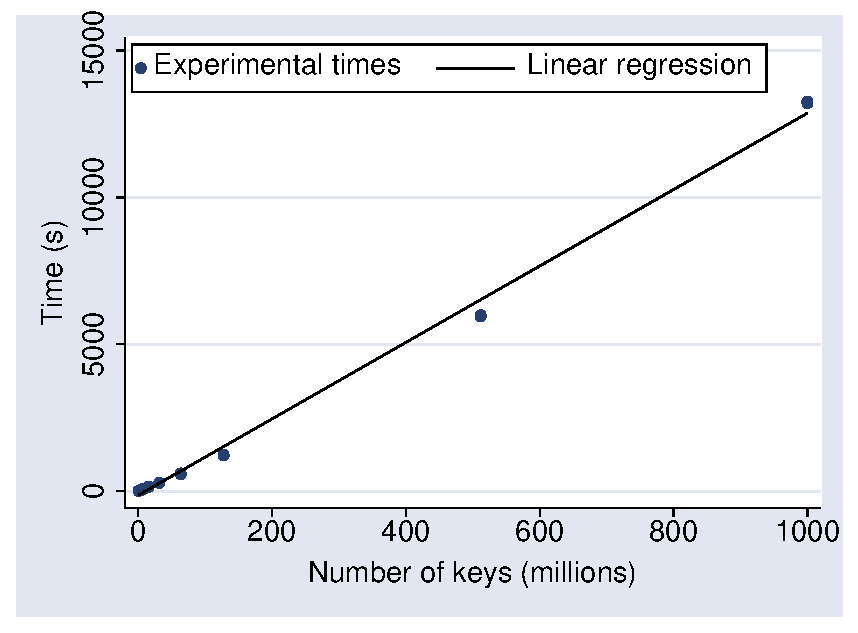
\includegraphics{figs/brz_temporegressao.eps}}}
%   \end{minipage}
%     \caption{Time versus number of keys in $S$. The solid line corresponds to 
% a linear regression model.}
% %obtained from the experimental measurements.}
%     \label{fig:temporegressao}
% \end{figure*}

Table~\ref{tab:medias} presents the runtime average for each $n$,
the respective standard deviations, and 
the respective confidence intervals given by 
the average time $\pm$ the distance from average time
considering a confidence level of $95\%$.
Observing the runtime averages one sees that 
the algorithm runs in expected linear time, 
as shown in~\cite{bkz05}. 

\vspace{-2mm}
\begin{table*}[htb]
\begin{center}
{\scriptsize
\begin{tabular}{|c|c|c|c|c|c|c|c|}
\hline
$n$ (millions)  & 1                 & 2                    & 4                  & 8                  & 16      & 32 \\
\hline
Average time (s)& $6.1 \pm 0.3$ & $12.2 \pm 0.6$   & $25.4 \pm 1.1$ & $51.4 \pm 2.0$ & $117.3 \pm 4.4$ & $262.2 \pm 8.7$\\
SD (s)          & $2.6$           & $5.4$              & $9.8$            & $17.6$           & $37.3$            & $76.3$  \\
\hline
\end{tabular}
\vspace{-1mm}
}
\end{center}
\caption{Internal memory based algorithm: average time in seconds for constructing a MPHF,
the standard deviation (SD), and the confidence intervals considering
a confidence level of $95\%$.}
\label{tab:medias}
\vspace{-4mm}
\end{table*}

% \enlargethispage{\baselineskip}
% \begin{table*}[htb]
% \begin{center}
% {\scriptsize
% (a)
% \begin{tabular}{|c|c|c|c|c|c|c|c|}
% \hline
% $n$ (millions)  & 1                 & 2                    & 4                  & 8                  & 16                 & 32 \\
% \hline
% Average time (s)& $6.119 \pm 0.300$ & $12.190 \pm 0.615$   & $25.359 \pm 1.109$ & $51.408 \pm 2.003$ & $117.343 \pm 4.364$ & $262.215 \pm 8.724$\\
% SD (s)          & $2.644$           & $5.414$              & $9.757$            & $17.627$           & $37.333$            & $76.271$  \\
% \hline
% \end{tabular}
% \\[5mm]  (b)
% \begin{tabular}{|l|c|c|c|c|c|}
% \hline
% $n$ (millions)   & 1                  & 2                  & 4                  & 8                   & 16             \\
% \hline % Part.      16 \%                 16 \%                 16 \%                18 \%                 20\%           
% Average time (s) & $6.927 \pm 0.309$  & $13.828 \pm 0.175$ & $31.936 \pm 0.663$ & $69.902 \pm 1.084$  & $140.617 \pm 2.502$  \\
% SD               & $0.431$            & $0.245$            & $0.926$            & $1.515$             & $3.498$         \\
% \hline
% \hline
% $n$ (millions)   & 32                  & 64                   & 128                    & 512                  & 1000            \\
% \hline % Part.      20 \%                 20\%                  20\%                      18\%                    18\%
% Average time (s) & $284.330 \pm 1.135$ & $587.880 \pm 3.945$  & $1223.581 \pm 4.864$   & $5966.402 \pm 9.465$ & $13229.540 \pm 12.670$  \\
% SD               & $1.587$             & $5.514$              & $6.800$                & $13.232$             & $18.577$            \\
% \hline
% \end{tabular}
% }
% \end{center}
% \caption{The runtime averages in seconds, 
% the standard deviation (SD), and
% the confidence intervals given by the average time $\pm$ 
% the distance from average time considering 
% a confidence level of $95\%$.}
% \label{tab:medias}
% \end{table*}

\enlargethispage{2\baselineskip}
Figure~\ref{fig:bmz_temporegressao} 
presents the runtime for each trial. In addition, 
the solid line corresponds to a linear regression model 
obtained from the experimental measurements.
As we can see, the runtime for a given $n$ has a considerable 
fluctuation. However, the fluctuation also grows linearly with $n$.

\begin{figure}[htb]
\vspace{-2mm}
\begin{center}
\scalebox{0.4}{\includegraphics{figs/bmz_temporegressao}}
\caption{Time versus number of keys in $S$ for the internal memory based algorithm.
The solid line corresponds to a linear regression model.}
\label{fig:bmz_temporegressao}
\end{center}
\vspace{-6mm}
\end{figure}

The observed fluctuation in the runtimes is as expected; recall that this
runtime has the form~$\alpha nZ$ with~$Z$ a geometric random variable with
mean~$1/p=e$.  Thus, the runtime has mean~$\alpha n/p=\alpha en$ and standard
deviation~$\alpha n\sqrt{(1-p)/p^2}=\alpha n\sqrt{e(e-1)}$. 
Therefore, the standard deviation also grows 
linearly with $n$, as experimentally verified 
in Table~\ref{tab:medias} and in Figure~\ref{fig:bmz_temporegressao}.

%\noindent-------------------------------------------------------------------------\\
%Comentario para Yoshi: Nao consegui reproduzir bem o que discutimos 
%no paragrafo acima, acho que vc conseguira justificar melhor :-). \\
%-------------------------------------------------------------------------\\
